% English version of paper/ja_v3/05_手法.md (ver3 draft 2, 2026-11-17). Following Ishii et al. 2022, the method section opens with the motivation, linking each analysis result to one design decision, and states the scope ("Our goal is not ... but ...") before the definition. The weight-table decomposition and episode figures moved to the Supplementary Information (Figs. S7, S8); the AFEW evaluation-run values moved to Sect. 6.3.
\FloatBarrier
\section{Method: emotion-wise reliability-weighted late fusion}\label{sec:method}

\subsection{Motivation}\label{sec:idea}
The idea of the proposal was conceived after seeing outputs of the evaluation run of distillation in Sect.~\ref{sec:analysis}, and its form was fixed on provisional-target computations (Sect.~\ref{sec:hp}); the (C13) aggregation of Sect.~\ref{sec:rq1b-margin} was set up after the method had been fixed. Below we state the three design decisions and the results that correspond to each.

First, the goal of the method is to raise the UAR of the pseudo-labels. In the (C13) aggregation set up later, every variant whose UAR rose also had pseudo-labels with higher UAR than the classifier before retraining, and none of the 173 and 184 variants with a negative advantage rose (Sect.~\ref{sec:rq1b-margin}).

Second, the weights differ by classifier and emotion, whereas the pseudo-labels of distillation, (D0), multiply the three classifiers' probabilities with equal weights. In provisional-target computations run to design the method (Sect.~\ref{sec:settings}; each of the four corpora as a provisional target with two of the remaining corpora as sources, 30 repetitions each), the classifier-by-emotion reliabilities (Sect.~\ref{sec:method-def}) measured with all candidate labels were highest for visual on all four emotions of AFEW and for text on all four of MELD, for visual on Happy and audio on the others in IEMOCAP, and changed with the emotion in MOSEI (Fig.~\ref{fig:idea}). We therefore use 12 weights, one per classifier and emotion. In the (C13) aggregation set up later, the corpus's strongest modality also differed across corpora (visual on AFEW, audio on IEMOCAP, visual on MOSEI, text on MELD), and retraining the classifier of the strongest modality on pseudo-labels from the other two modalities gave negative gains in point estimates in all eight cases (Sect.~\ref{sec:rq1b-margin}).

\begin{figure}[t]
\centering
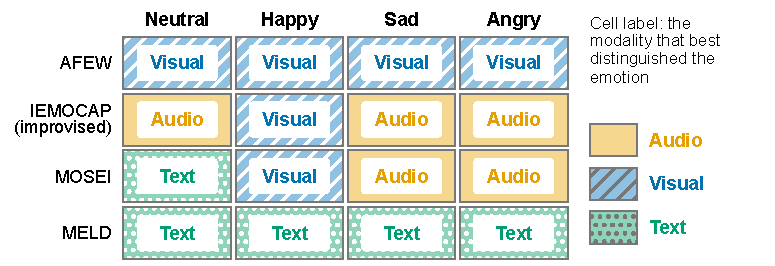
\includegraphics[width=\textwidth]{figures/fig_prop_idea_en.pdf}
\caption{For each corpus and emotion, the modality with the highest reliability. Values are reliabilities used to design the method (provisional-target computations, all candidate labels, K = 5, mean of 30 repetitions), not values of the evaluation run}\label{fig:idea}
\end{figure}

Third, measuring all 12 weights on the K target labels would determine each weight from only K utterances per emotion. In the same provisional-target computations, we built two classifier-by-emotion reliability tables, one measured on the sources and one on all candidate labels of the provisional target, and found that splitting the weights into two parts allows each part to be measured on different data (values in Supplementary Information S5). The ranking of classifier strengths (mean reliability over the four emotions) changed across corpora. For every corpus and K, the strongest modality by source-measured strength differed from that on all candidate labels in more than half of the repetitions, and the K-label strengths agreed in more repetitions than the source-measured ones in 11 of the 12 combinations of corpus and K. The classifier-by-emotion component left after removing classifier effects, emotion effects and a non-additivity term, by contrast, correlated positively between the source table and the candidate-label table. We therefore measure strengths on the K target labels and per-emotion profiles on the labelled source corpora.

Our goal is not to build a new fusion architecture that learns per-utterance weights, but to set, with only a few target labels, weights that raise the UAR of the pseudo-labels while fitting only three quantities (one strength per classifier) on the K labels.

\subsection{Definition}\label{sec:method-def}
The proposal weights the predictions of the classifiers that make the product of (C1) (the product components) with a classifier-by-emotion reliability table and turns the fused predictions into pseudo-labels. The table is the sum of strengths and per-emotion profiles (Fig.~S7).

The reliability is defined on the scores of each classifier. With probabilities $p_m(i\mid x)$ of classifier $m$ for emotion $i$, the centred log-probability is the score $z_m(i\mid x)=\log p_m(i\mid x)-\frac14\sum_j\log p_m(j\mid x)$, and
\begin{equation}\label{eq:rel}
d_m(i)=\max\!\big(0,\sqrt2\,\Phi^{-1}(A_m(i))\big),\quad A_m(i)\in[0.02,0.98],
\end{equation}
where $A_m(i)$ is the mean over emotions $j\neq i$ of the area under the ROC curve (AUC) separating utterances of true emotion $i$ from those of $j$ by $z_m(i\mid\cdot)$, and $\Phi^{-1}$ is the standard normal quantile function ($d_m(i)\le 2.90$). Because the ranks of scores do not change when intercepts are shifted, $d_m(i)$ depends neither on the classifier's intercepts nor on the target's emotion proportions. The mean over the four emotions is the strength $L_m$, and $d_m(i)-L_m$ is the per-emotion profile.

The strengths are measured on the K labels. The K labels are split into five subsets per emotion; for each subset $f$, the product components are retrained by the procedure of (C1) on the K labels without subset $f$ and assign probabilities to subset $f$; the reliabilities of Eq.~(\ref{eq:rel}) computed from the five subsets' probabilities are averaged over emotions to give $L^{K}_m$. Because $L^{K}_m$ is noisy for small K, a default strength $L^{0}_m$ (the mean of the three $L^{K}_m$ or the strength measured on the sources) is mixed in with weight $n_0$:
\begin{equation}
L_m=\frac{n\,L^{K}_m+n_0\,L^{0}_m}{n+n_0},\qquad n=4K.
\end{equation}

The profiles are measured on the source corpora. Within each source $s$, $d^{\mathrm{in}}_{s,m}(i)$ is measured by speaker-split five-fold cross-validation, and a classifier trained on all of $s$ is applied to another source $t$ to give $d^{\mathrm{out}}_{s\to t,m}(i)$. The share of modality $m$'s reliability that carries over to other corpora is $\eta_m=\sum_{s\to t}\sum_i d^{\mathrm{out}}_{s\to t,m}(i)/\sum_{s\to t}\sum_i d^{\mathrm{in}}_{s,m}(i)$ (clipped to $[0,1.5]$), and
\begin{equation}
d^{\mathrm{src}}_m(i)=\eta_m\frac{1}{|S|}\sum_s d^{\mathrm{in}}_{s,m}(i),\qquad r^{\mathrm{src}}_m(i)=d^{\mathrm{src}}_m(i)-\frac14\sum_j d^{\mathrm{src}}_m(j)
\end{equation}

The reliability table combines strengths and profiles, and the fused predictions give the pseudo-labels. The table is $T(m,i)=\max(0,L_m+\beta\,r^{\mathrm{src}}_m(i))$ ($\beta=1$ uses the profiles, $\beta=0$ does not); dividing by its mean gives weights $\Omega(m,i)=T(m,i)/(\frac{1}{12}\sum_{m',i'}T(m',i'))$, and the scores are summed per emotion, $s(i\mid x)=\sum_m \Omega(m,i)\,z_m(i\mid x)$. Because emotion-specific weights can shift predictions towards some emotions, intercepts $c$ are shifted without labels so that the mean of $\mathrm{softmax}(s(\cdot\mid x)+c)$ over candidates equals the mean of the product's probabilities (fixed-point iteration). The fused decision at estimation time is $\arg\max_i(s(i\mid x)+c_i)$. We attach $q(i\mid x)=\mathrm{softmax}_i(s(i\mid x)+c_i)$ to the candidates as pseudo-labels (soft labels) and retrain the AVT classifier (AV for CREMA-D) with the loss of (C1) (Sect.~\ref{sec:rq1b-compare}). Because the fused predictions carry information of all three modalities, the retrained classifier is AVT, which takes all three features; comparisons of estimation-time decisions (group D) do not depend on it. Audio, visual and text classifiers retrained on the proposal's pseudo-labels were not computed (Sect.~\ref{sec:limitations}). $\rho$ and $a$ are borrowed from the values chosen for the product's pseudo-labels.

\subsection{Hyperparameter selection on source-corpus episodes}\label{sec:hp}
The hyperparameters ($n_0\in\{0,20,80,\infty\}$, $\beta\in\{0,1\}$ and the two default strengths; 16 settings, 14 distinct) were selected, per evaluation target and K, by the highest mean UAR on the test folds of the provisional targets over three episodes in which each source corpus served in turn as a provisional target with the other two as sources (3 corpora $\times$ 5 folds $\times$ 2 seeds = 30 repetitions; Fig.~S8). No data of the evaluation target enter any episode. All selected settings had $\beta=1$, and $n_0$ was 0 in 8 of 12 conditions and 20 in the other four. The setting $n_0=\infty$, $\beta=0$ with the mean default strength gives the same decisions as the product. For CREMA-D, the hyperparameters ($n_0=0$, $\beta=1$) and $\rho$ and $a$ for the AV classifier were selected on the repetitions of a six-corpus provisional-target computation (the four corpora plus CREMA-D and RAVDESS) that do not involve CREMA-D. The form of the method was fixed after seeing the provisional-target runs, and the evaluation was computed once; the idea of the proposal was conceived after seeing outputs of the evaluation run of (C1)--(C13), and CREMA-D was added to the evaluation after its values had been seen in the six-corpus provisional runs (Sect.~\ref{sec:limitations}).
